\documentclass{article}

\usepackage{amsmath}
\usepackage{mathtools}
\usepackage{subfigure}
\usepackage{enumerate}
\setlength\parindent{0pt}

\setlength{\textwidth}{6.2in}
\setlength{\oddsidemargin}{0.0in}
\setlength{\evensidemargin}{0in}
\setlength{\textheight}{8.9in}
\setlength{\voffset}{-1in}
\setlength{\headsep}{26pt}
\setlength{\parindent}{0pt}
\setlength{\parskip}{5pt}

\begin{document}

% Introduction
\section{Introduction}
When a model is called ``higher order", we usually associate it with being more accurate than a first order model.  This is not always the case.  Adding complexity to a model does not necessarily improve it, as is demonstrated in the class of higher order traffic models developed with the intention of improving the first order traffic model proposed by Lighthill and Whitham (1955) and Richards (1956).  As Daganzo observes in his paper, \\

``A new theory (e.g. relativity) is deemed successful if it explains previously unexplained phenomena, plus everything else that was correctly explained with the theory it intends to replace (e.g. Newtonian physics).  In the case of traffic flow, the new theories (high-order fluid models) fail to explain the behavior of traffic at the end of a queue (unlike the simpler, older LWR model; which explains it perfectly)." \\

In this paper we examine the second order traffic model developed by Payne (1971) and Whitham (1974) which was meant to improve how the LWR model explains traffic behavior near shocks.  Their model takes its form from equations used to describe compressible fluid dynamics.  Unfortunately, cars and fluid particles have some fundamental differences which make the model actually perform worse than the LWR model in certain cases.  For example, by smoothing out discontinuities, the PW model predicts negative velocities, which is clearly a problem.  \\

In addition to considering the PW model, we also take a look a more successful model proposed by Aw and Rascle (2000).  These authors challenge some of the assumptions of the PW model and suggest the use of a convective derivative to fix the problem of negative velocities.  In order to verify that their model is valid, they test their new model against criteria they claim any reasonable model will satisfy.  

% LWR Model
\section{LWR Model}
We can start by considering a first order (one equation) model of traffic flow on a one-way highway without any exits, entrances, or passing.  In this case, we can expect that the number of cars will be conserved, so we can use the equation for conservation of mass (with density $\rho$ and velocity $v$):

\begin{enumerate}[(a)]
\item Integral form of equation: $\displaystyle \frac{d}{dt} \int_{x_1}^{x_2} \rho \, dt = -\Big[ f( \rho ) \Big]_{x_1}^{x_2}$
\item Differential form of equation: $\rho_t + f( \rho )_x = 0$
\begin{enumerate}[i]
\item Light traffic: $\rho_t + (\rho v)_x = 0$
\item Congested traffic: $\rho_t + \Big( \rho V(\rho) \Big)_x = 0$ (LWR model)
\end{enumerate}
\end{enumerate}

The LWR behaves well macroscopically, but it does have some flaws.  For example, it assumes cars change their velocity instantaneously as they travel through shocks.  One way to eliminate shocks would be to add a diffusion term: $\rho_t + \Big( \rho V(\rho) \Big)_x = \mu \rho_{xx}$.  This term is meant to account for the drivers awareness of the road ahead.  However, this model can be shown to predict negative velocities in some instances, which is obviously wrong.

% PW Model
\section{PW Model}

% PW Model: Theory
\subsection{Theory}
Another approach to improving the LWR model would be to use a second order (two equation) model. Since cars can be thought of as a compressible gas, we can use equations for conservation of mass (above) and conservation of momentum, $\rho v$, used to model compressible gas flow:

\begin{enumerate}[(a)]
\item Integral form of equation: $\displaystyle \frac{d}{dt} \int_{x_1}^{x_2} \rho v \, dt = -\Big[ f( \rho v ) \Big]_{x_1}^{x_2}$
\item Differential form of equation: $(\rho v)_t + f( \rho v )_x = (\rho v)_t + \Big( \rho v^2 + \rho \Big)_x = 0$
\end{enumerate}

We can rewrite the second equation in terms of velocity instead of momentum: $v_t + v v_x + \dfrac{p'(\rho)}{\rho} \rho_x = 0$. \\

The PW model is a modification of these equations for conservation of mass and conservation of momentum in gas dynamics, with added relaxation and diffusion terms: 

\[ \left\{ \begin{matrix*}[l] & \rho_t + (\rho v)_x = 0 \\[1ex] & v_t + v v_x + \dfrac{p'(\rho)}{\rho} \rho_x = \dfrac{V(\rho) - v}{\tau} + \mu v_{xx} \end{matrix*} \right. \]

At first glance, this seems like a reasonable model.  However, there a couple of fundamental differences between gas particles and cars that could be problematic.  For example, as pointed out by Daganzo, ``a fluid particle responds to stimuli from the front and from behind, but a car is an anisotropic particle that mostly responds to frontal stimuli."  If we consider the eigenvalues of the Jacobian matrix of the linearized system, we see that one of the eigenvalues, $\lambda_2 = v + \sqrt{p'(\rho)}$, represents information traveling faster than the velocity of cars in the system.  This implies that traffic conditions are partially determined by what is going on behind.

% PW Model: Hugoniot Loci and Integral Curves
\subsection{Hugoniot Loci and Integral Curves}
Brisa

% AR Model
\section{AR Model}

% AR Model: Theory
\subsection{Theory}
Another issues with the PW model, as Aw and Rascle point out in their paper, is that there is no conservation of momentum in car traffic.  Instead, the term involving pressure is mean to represent an anticipation factor, or how a driver would react to a variation in the concentration of cars with respect to space.   However, what we should really be concerned with is the perspective of the driver, which is relative to a moving timeframe.  In this case, we should be using a convective derivative, $\partial_t + v \partial_x$, of the pressure.  The new model becomes:

\[ \left\{ \begin{matrix*}[l] & \rho_t + (\rho v)_x = 0 \\[1ex] & (v + p)_t + v (v + p)_x = 0 \end{matrix*} \right. \]

The second equation can also be rewritten as an equation for velocity: $v_t + \Big(v - \rho p'(\rho)\Big)v_x = 0$. \\

This updated model no longer conserves momentum.  Instead, it conserves the quantity $y = v + p(\rho)$, which we can see if we rearrange the second equation to a conservation form: $(\rho (v + p(\rho)))_t + (\rho v(v + p(\rho)))_x = 0$. While the authors admit that there is no obvious physical interpretation of this quantity, they claim that it is the most natural pair of conservative variables. \\

The authors also claim that their improved model satisfies the following important conditions:
\begin{enumerate}
\item The system is hyperbolic.
\item When solving the Riemann problem with bounded nonnegative data $(\rho, v)$, the density and velocity must remain nonnegative and bounded from above.
\item When solving the Riemann problem, no waves connecting any state to its left (behind it) can have a propagation speed greater than the velocity $v$.
\item The solution to the Riemann problem must agree with qualitative properties that drivers actually experience: braking produces shock waves and acceleration produces rarefaction waves.
\item Near a vacuum, the solution to the Riemann problem must be sensitive to the data.
\end{enumerate}

% AR Model: Hugoniot Loci and Integral Curves
\subsection{Hugoniot Loci and Integral Curves}
The AR model starts from the system
\begin{align}
&\partial_t\rho + \partial_x(\rho v) = 0, \label{AR:eq1}\\
&\partial_t \left(v + p(\rho )\right) + v\partial_x \left( v + p(\rho )\right) = 0\label{AR:eq1.5}
\end{align}
with $p(\rho) = \rho^\gamma$.

To find the Hugoniot loci and the integral curves, \cite{AwRascle2000} utilizes two different forms of this system. 
We will examine each of them in turn. What we will find is that the integral curves and the Hugoniot loci coincide, 
and furthermore that one of the waves is a contact discontinuity. Let us first consider the Hugoniot loci. 

\subsubsection{Hugoniot Loci}
In order to consider the Hugoniot loci for this system we must first write the system in conversation form. 
To accomplish this, note that multiplying the first equation by $(v + p(\rho ))$ and the second equation 
by $\rho$ gives us the two equations 
\begin{align*}
&(v + p(\rho ))\partial_t\rho + (v + p(\rho ))\partial_x(\rho v) = 0,  \\
&\rho\partial_t \left(v + p(\rho )\right) + \rho v\partial_x \left( v + p(\rho )\right) = 0.
\end{align*}
Adding these two equations gives
\begin{align}\label{AR:eq2}
\partial_t \left(\rho\left(v + p(\rho )\right)\right) + \partial_x \left( \rho v\left(v + p(\rho )\right)\right) = 0.
\end{align}
Then from (\ref{AR:eq1}) and (\ref{AR:eq2}) we have the system 
\begin{align*}
&\partial_t\rho + \partial_x(\rho v) = 0, \\
&\partial_t \left(\rho\left(v + p(\rho )\right)\right) + \partial_x \left( \rho v\left(v + p(\rho )\right)\right) = 0.
\end{align*}
This can be rewritten as $q_t + f(q)_x = $ by defining
\begin{align*}
q = \left[ \begin{matrix}
\rho \\ y
\end{matrix}\right], \hspace{0.3in}
f(q) = \left[ \begin{matrix}
v\rho \\
vy
\end{matrix}\right].
\end{align*}
where $y = \rho\left(v + p(\rho )\right)$.
The Rankine-Hugoniot condition tells us that 
\begin{align*}
s(q_*- q) = f(q_*) - f(q).
\end{align*}
Therefore, from this condition we get the two equations
\begin{align}
s(\rho_* - \rho) = v_*\rho_* - v\rho, \label{AR:eq3}\\
s(y_* - y) = v_*y_* - vy.\label{AR:eq4}
\end{align}
With a little rearranging and by plugging in for $y$, these two equations can be rewritten as
\begin{align}
&\rho_*(s - v_*) = \rho (s - v), \label{AR:eq5}\\
&\rho_*(s - v_*)\left(v_* + p(\rho_* )\right) = \rho(s - v)\left(v + p(\rho )\right).\label{AR:eq6}
\end{align}
From (\ref{AR:eq5}), we know that there are two cases: 

(a) $\rho_*(s - v_*) = \rho (s - v) = 0$. In this case we have that
\begin{align*}
s - v_* = s - v 
\end{align*}
except if one of the two densities, $\rho_*$, $\rho$ is zero. WHY DOES THIS NOT MATTER? Therefore, we can say that
\begin{align*}
v_* = v.
\end{align*}
Since the velocity does not change, this is a contact discontinuity. Using the fact that $v = v_*$ in (\ref{AR:eq4}) gives
\begin{align*}
y_*(s - v) = y(s - v).
\end{align*}
So, either $y = y_*$ or $s = v$. If $y = y_*$ we have a stationary point in the $Y = (\rho, y)$ plane, which does not 
describe a wave. Therefore, $s = v$. Note that we have no restrictions on $y$ other than its definition. 
Therefore this loci in the $Y$ plane is given by 
\begin{align*}
y = \rho ( v_* + p(\rho )).
\end{align*}
(b) $\rho_*(s - v_*) = \rho (s - v) \neq 0$. In this case, plugging this into (\ref{AR:eq6}) gives
\begin{align*}
\rho_*(s - v_*)\left(v_* + p(\rho_* )\right) &= \rho(s - v)\left(v + p(\rho )\right)\\
\rho(s - v)\left(v_* + p(\rho_* )\right) &= \rho(s - v)\left(v + p(\rho )\right)\\
v_* + p(\rho_* )&= v + p(\rho ).
\end{align*}
Therefore, the Hugoniot loci for this case in the Y plane are given by
\begin{align*}
y = v_* + p(\rho_* ),
\end{align*}
since $y = v + p(\rho )$ by definition. Note that solving (\ref{AR:eq3}) for $s$ gives
\begin{align*}
s = \frac{\rho_*v_* - \rho v}{\rho_* - \rho}.
\end{align*}
Using the fact that $v_* = v + p(\rho) - p(\rho_*)$, we get that
\begin{align*}
s = \frac{\rho_*\left( v + p(\rho) - p(\rho_*)\right)- \rho v}{\rho_* - \rho}
= v - \rho_*\frac{p(\rho ) - p(\rho_*)}{\rho - \rho_*}
\approx v - \rho p'(\rho)
\end{align*}
for $\rho_* \approx \rho$. 

In the $U = (\rho, v)$ plane these loci become (a) $v = v_*$, $\rho$ free, and (b) $v = v_* + p(\rho_* ) - p(\rho )$.
 In the $M = (\rho, \rho v)$ plane these loci become (a) $\rho v = \rho_* v_*$, $\rho$ free, 
 and (b) $\rho v = \rho \left( v_* + p(\rho_*)\right) - \rho p(\rho))$. Figure \ref{fig:AR_curves} shows the Hugoniot loci 
 in the different planes. TODO: ADD PARAMETERS USED FOR FIGURES? OR, WILL INCLUDING THE CODE MAKE THAT REDUNDANT? 
 IF WE ADD PARAMETERS, MAYBE THE BEST PRESENTATION WOULD BE IN A TABLE?

\begin{figure}[h!]
 \centering
 \subfigure[$\lambda_1$-curves in the U plane.]{
  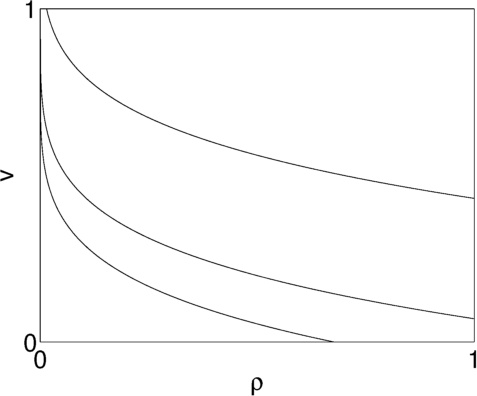
\includegraphics[width=45mm]{../MatlabCode/Images/HLIC_U_lamb1.jpg}
   }
 \subfigure[$\lambda_2$-curves in the U plane.]{
  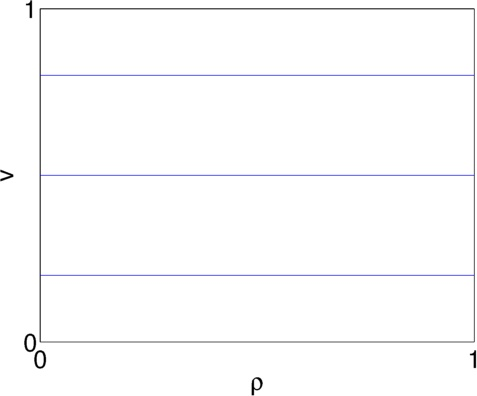
\includegraphics[width=45mm]{../MatlabCode/Images/HLIC_U_lamb2.jpg}
   }
 \subfigure[$\lambda_1$-curve and $\lambda_2$-curve in the U plane passing through
  the point $(\rho_*, v_*)$ denoted by the red point.]{
  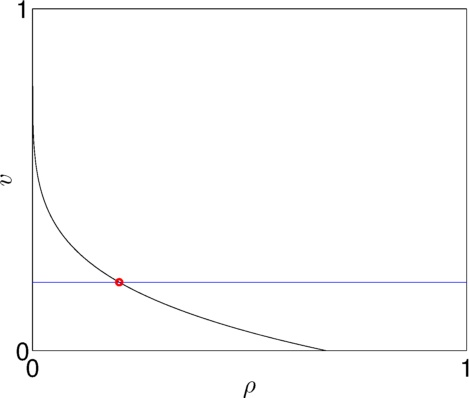
\includegraphics[width=45mm]{../MatlabCode/Images/HLIC_U.jpg}
   }
    \subfigure[$\lambda_1$-curves in the M plane.]{
  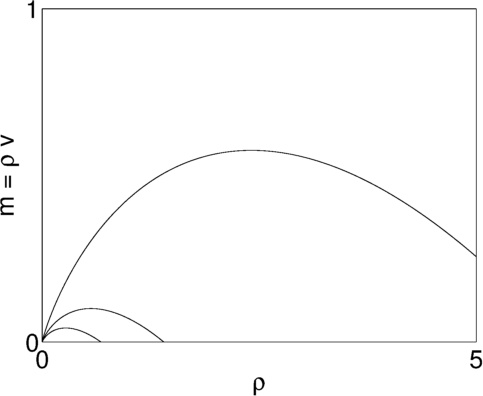
\includegraphics[width=45mm]{../MatlabCode/Images/HLIC_M_lamb1.jpg}
   }
 \subfigure[$\lambda_2$-curves in the M plane.]{
  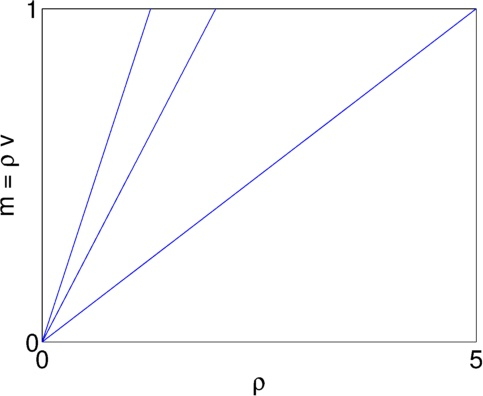
\includegraphics[width=45mm]{../MatlabCode/Images/HLIC_M_lamb2.jpg}
   }
 \subfigure[$\lambda_1$-curve and $\lambda_2$-curve in the M plane passing through 
 the point $(\rho_*,m_*)$ denoted by the red point.]{
  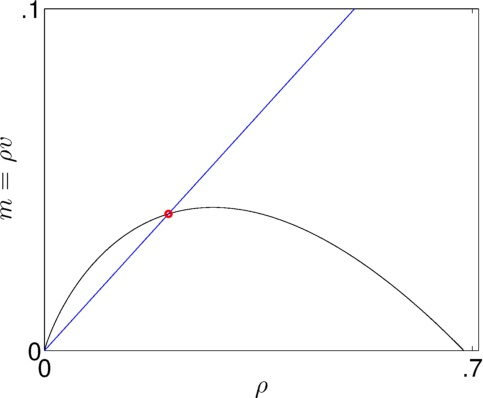
\includegraphics[width=45mm]{../MatlabCode/Images/HLIC_M.jpg}
   }
       \subfigure[$\lambda_1$-curves in the Y plane.]{
  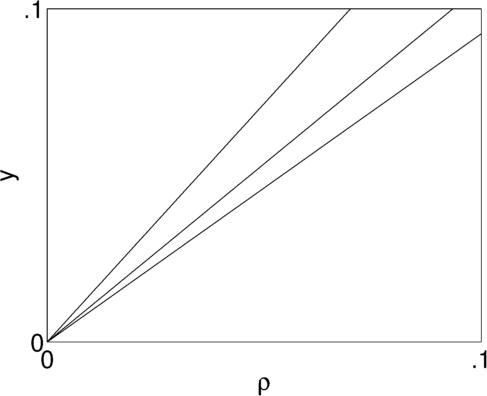
\includegraphics[width=45mm]{../MatlabCode/Images/HLIC_Y_lamb1.jpg}
   }
 \subfigure[$\lambda_2$-curves in the Y plane.]{
  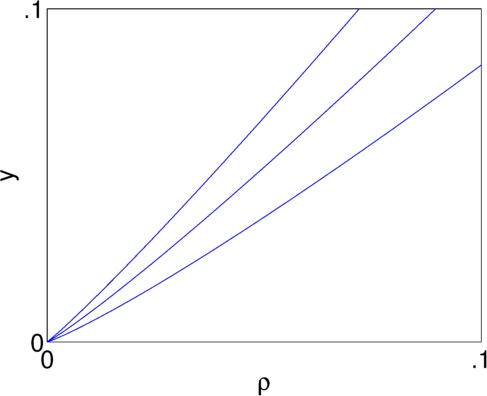
\includegraphics[width=45mm]{../MatlabCode/Images/HLIC_Y_lamb2.jpg}
   }
 \subfigure[$\lambda_1$-curve and $\lambda_2$-curve in the Y plane passing through 
 the point $(\rho_*, y_*)$ denoted by the red point.]{
  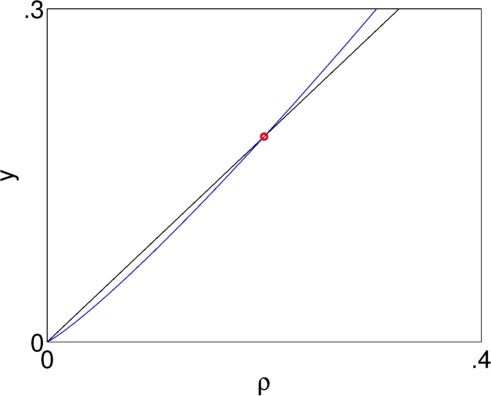
\includegraphics[width=45mm]{../MatlabCode/Images/HLIC_Y.jpg}
   }
 \caption[Optional caption for list of figures]
 {Figures of the Hugonio loci and integral curves for $\lambda_1$ and $\lambda_2$ 
 in each of the different planes. Since the loci and integral curves coincide, they are 
 both simply called the ``curves'' in the captions of the above figures. 
 Figures (c), (f), (i) show both curves for a given point in each plane.}
  \label{fig:AR_curves}
\end{figure}

\subsubsection{Integral Curves}
In order to consider the integral curves for this system \cite{AwRascle2000} 
works from the system
\begin{align*}
&\partial_t \rho + \partial_x (\rho v) = 0 \\ 
&\partial_t v + \left(v - p'(\rho)\rho\right)\partial_x v = 0,
\end{align*}
where the second equation is found by multiplying (\ref{AR:eq1}) 
by $p'(\rho)$ and subtracting it from (\ref{AR:eq1.5}). 
This can be rewritten as $q_t + Aq_t = 0$ by defining
\begin{align*}
q = \left[ \begin{matrix}
\rho \\ v
\end{matrix}\right] , \hspace{0.3in}
A = \left[ \begin{matrix}
v & \rho \\
0 & v - p'(\rho ) \rho
\end{matrix}\right].
\end{align*}
The eigenvalues of $A$ are $\lambda_1 = v - p'(\rho ) \rho$ and 
$\lambda_2 = v$. Note that since $p(\rho ) = \rho^{\gamma}$ 
and $\rho \geq 0$, $\lambda_1 < \lambda_2$ so long as $\rho \neq 0$. 
Also note that if $\rho = 0$ then $A$ is no longer 
hyperbolic. The eigenvectors of $A$ are
\begin{align*}
r_1 = \left[ \begin{matrix}
1 \\ - p'(\rho )
\end{matrix}\right], \hspace{0.3in}
r_2 = \left[ \begin{matrix}
1 \\ 0
\end{matrix}\right].
\end{align*}
Using equation (13.24) from \cite{LeVeque2002} with $\alpha = 1$ tells us 
that the integral curves can be found by considering $q'(\xi ) = r_p$. 
For $p = 1$ this gives us the two equations
\begin{align*}
&\rho'(\xi ) = 1 \\
&v'(\xi ) = - p'(\rho ),
\end{align*}
which can be solved to find that we have parameratized our curve by $\rho$, 
and $v = - p'(\rho ) + c_1$ while $\rho$ is free, where $c_1$ is a constant. 
Since for a given point $(\rho_*, v_*)$ when $\rho = \rho_*$ we want 
$v = v_*$, we get that $c_1 = v_* + p'(\rho_*)$. Thus, the integral curve 
is given by 
\begin{align*}
v = v_* + p'(\rho_*) - p'(\rho ).
\end{align*}
This coincides with the Hugoniot loci from case (b). For $p = 2$, we get the 
two equations
\begin{align*}
&\rho'(\xi ) = 1 \\
&v'(\xi ) = 0,
\end{align*}
which can be solved to find that we have parameratized our curve by $\rho$, 
and that $v$ is a constant. Therefore, $v = v_*$ and $\rho$ is free. 
This coincides with the Hugoniot loci from case (a).

\subsubsection{Regions of Validity}
Restrictions on the way that $\lambda$ must vary across a wave allow us to identify the regions of the Hugoniot loci and integral curves that are valid for any given point. When traveling across a shock from a left state, $q_l$, to a right state $q_r$, $\lambda$ must decrease. When traveling across a rarefaction wave from a left state, $q_l$, to a right state $q_r$, $\lambda$ must increase. 

\begin{figure}[h!]
 \centering
 \subfigure[$\lambda_1$-curves with contours of $\lambda_1$ in the U plane.]{
  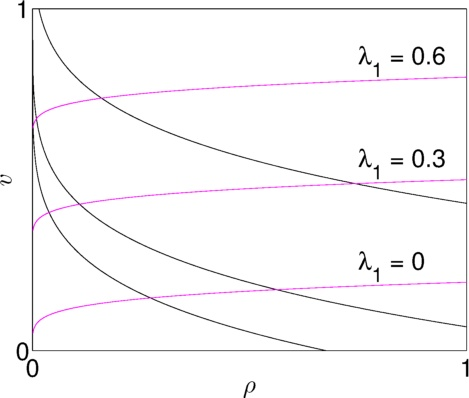
\includegraphics[width=45mm]{../MatlabCode/Images/Validity_U.jpg}
   }
    \subfigure[Valid waves for the point $q_l$ in the U plane.]{
  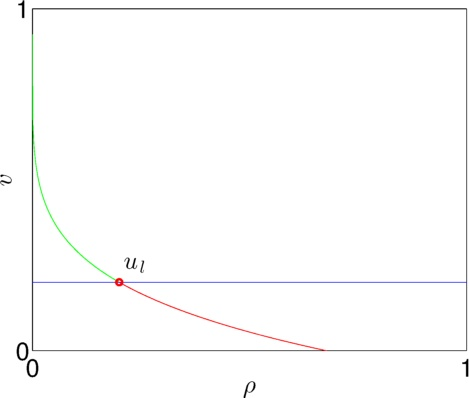
\includegraphics[width=45mm]{../MatlabCode/Images/Validity_U_ql.jpg}
   }
    \subfigure[Valid waves for the point $q_r$ in the U plane.]{
  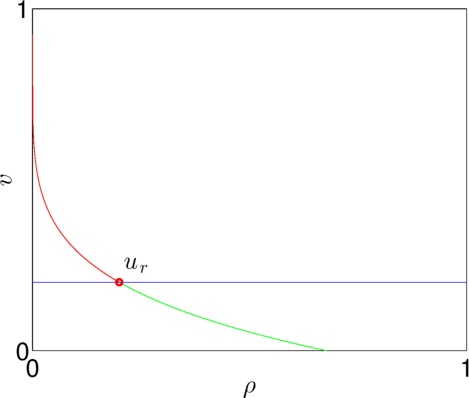
\includegraphics[width=45mm]{../MatlabCode/Images/Validity_U_qr.jpg}
   }
    \subfigure[$\lambda_1$-curves with contours of $\lambda_1$ in the M plane.]{
  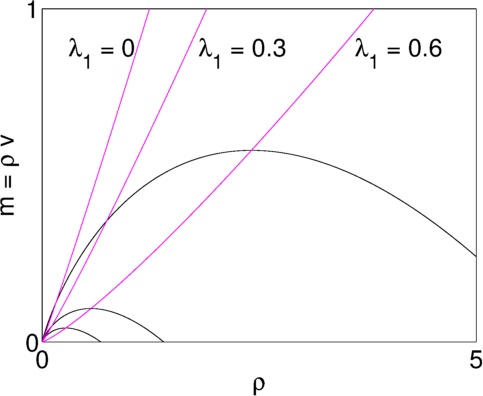
\includegraphics[width=45mm]{../MatlabCode/Images/Validity_M.jpg}
   }
 \subfigure[Valid waves for the point $q_l$ in the M plane.]{
  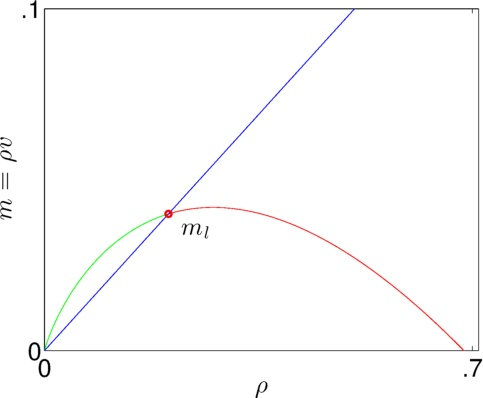
\includegraphics[width=45mm]{../MatlabCode/Images/Validity_M_ql.jpg}
   }
 \subfigure[Valid waves for the point $q_r$ in the M plane.]{
  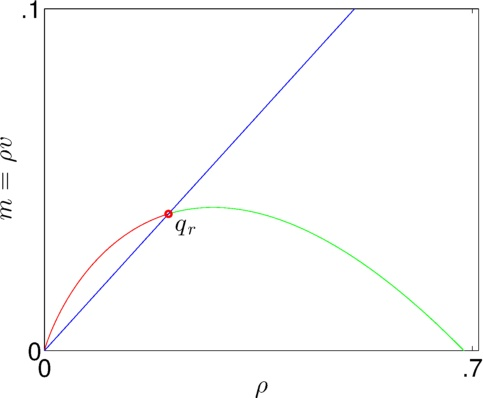
\includegraphics[width=45mm]{../MatlabCode/Images/Validity_M_qr.jpg}
   }
 \caption[Optional caption for list of figures]
 {Figures showing the calculation of the valid waves for a given point. Figures (a)
  and (d) show the $\lambda_1$ curves in black with the $\lambda_1$ contours 
  in magenta. The other figures show valid shocks in red and valid rarefaction 
  waves in green. The contact discontinuity is shown in blue.}
   \label{fig:AR_validity}
\end{figure}

Therefore, it is important to take into account the contour lines of $\lambda$ when 
looking at the loci and integral curves. Figures \ref{fig:AR_validity}(a) and 
\ref{fig:AR_validity}(d) show the $\lambda_1$-curves in the $U$ and $M$ planes,
with the contour lines of $\lambda_1$ shown in magenta. This information is used
to determine which areas of the $\lambda_1$ curves are valid shock waves and which
are valid rarefaction waves. The rest of the subfigures show the regions of validity for 
specific points $q_*$, depending on whether $q_* = q_l$ or $q_* = q_r$. For these plots,
$q_* = (\rho_*,v_*) = (0.2, 0.2)$. Note that the contact discontinuity is valid
anywhere in the plane. 

% Examples
\section{Examples}

\begin{figure}[h!]
 \centering
 \subfigure[Solution from the AR model.]{
  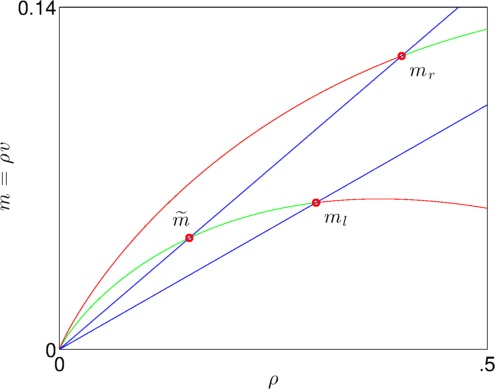
\includegraphics[width=70mm]{../MatlabCode/Images/AR_example1.jpg}
   }
% TODO: add subfigure for example1 in PW
 \caption[Optional caption for list of figures]
 {Solutions to the Riemann problem for example 1 from the AR and PW models.}
  \label{fig:example1}
\end{figure}

\begin{figure}[h!]
 \centering
 \subfigure[Solution from the AR model.]{
  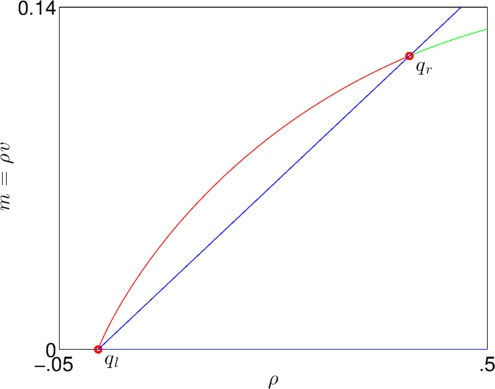
\includegraphics[width=70mm]{../MatlabCode/Images/AR_example2.jpg}
   }
% TODO: add subfigure for example2 in PW
 \caption[Optional caption for list of figures]
 {Solutions to the Riemann problem for example 2 from the AR and PW models.}
  \label{fig:example2}
\end{figure}

\begin{table}[t]
\caption{Initial values used in examples 1 and 2.}
\begin{center}
\begin{tabular}{| c | c c |}
\hline
& Example 1 & Example 2\\
\hline
$v_l$ & 0.2 & 0 \\
$\rho_l$ & 0.3 & 0\\
$v_r$ & 0.3 & 0 .3\\
$\rho_r$ & 0.4 & 0.4\\
\hline
\end{tabular}
\end{center}
 \label{table:1}
\end{table}

Reproducing the Riemann problems found in \cite{AwRascle2000}, we consider two different examples. The variables used in these two examples are shown in Table \ref{table:1}. Note that in example 1, shown in Figure \ref{fig:example1}, the transition from $m_l = (\rho_l, v_l\rho_l)$ to $m_r = (\rho_r, v_r\rho_r)$ is first a shock and then a contact discontinuity. The middle state is denoted by $\tilde{m}$ in the figure. In example 2, show in Figure \ref{fig:example2}, the transition from $m_l = (\rho_l, v_l\rho_l)$ to $m_r = (\rho_r, v_r\rho_r)$ is a rarefaction wave, and there is no middle state.

\bibliography{Draft}{}
\bibliographystyle{plain}
\end{document}